%%%%%%%%%%%%%%%%%%%%%%%%%%%%%%%
%   Figures for chapter 4
%%%%%%%%%%%%%%%%%%%%%%%%%%%%%%%

\newcommand{\figMeasureIntelligence}{
    \begin{figure}
        \centering
        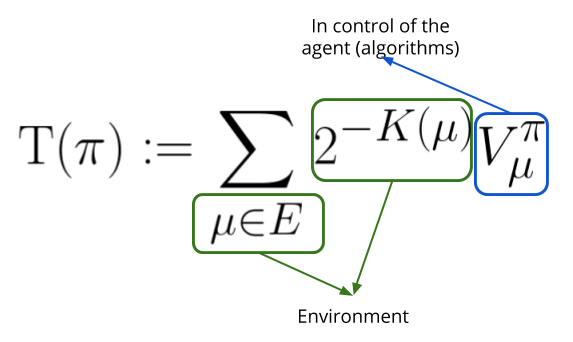
\includegraphics[width=0.4\textwidth]{./chapters/chapter_4/imgs/img_ch4_measure_tasks_agents.png}
        \caption{Measure of intelligence proposed by \cite{UniversalIntelligence}}
        \label{fig:ch4_measure_of_intelligence}
    \end{figure}
}

\newcommand{\figTerrainParameterizationZero}{
    \begin{figure}[!ht]
        \centering
        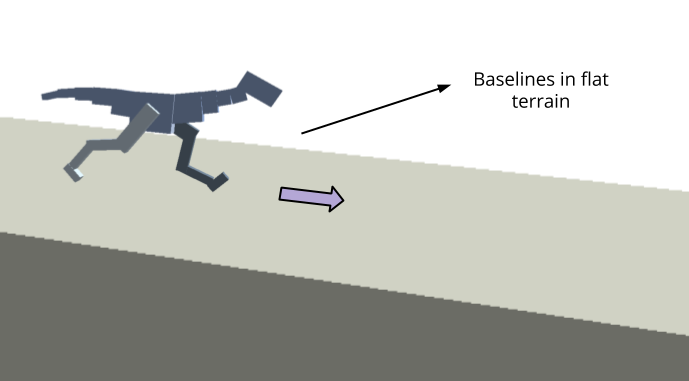
\includegraphics[width=0.9\textwidth]{./chapters/chapter_4/imgs/img_ch4_terrain_parameterization_0.png}
        \caption{Base experiments to test the baseline implementations}
        \label{fig:ch4_terrain_parameterization_zero}
    \end{figure}
}

\newcommand{\figTerrainParameterizationOne}{
    \begin{figure}[!ht]
        \centering
        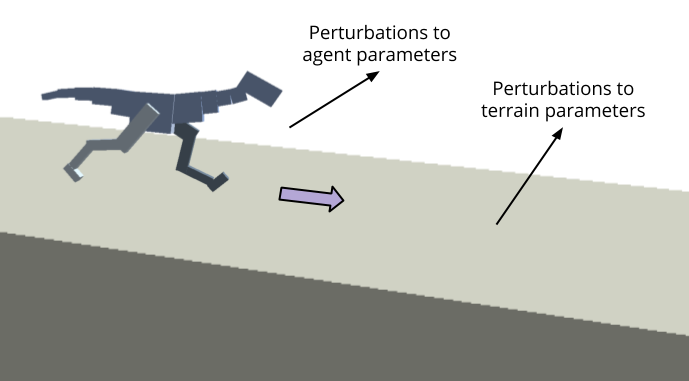
\includegraphics[width=0.9\textwidth]{./chapters/chapter_4/imgs/img_ch4_terrain_parameterization_1.png}
        \caption{A first variation of the environments, modifying the terrain and agents parameters}
        \label{fig:ch4_terrain_parameterization_one}
    \end{figure}
}

\newcommand{\figTerrainParameterizationTwo}{
    \begin{figure}[!ht]
        \centering
        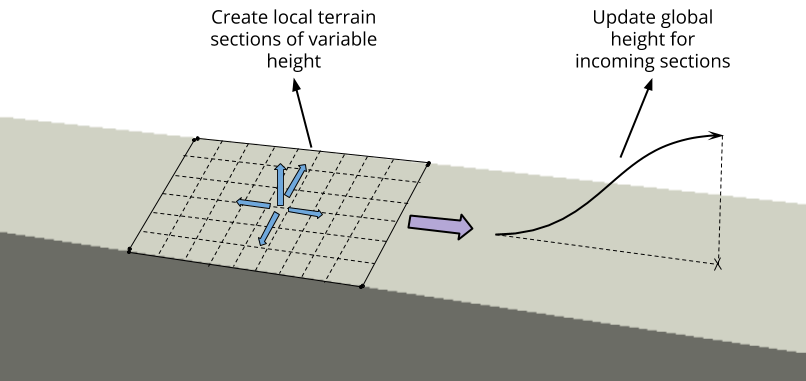
\includegraphics[width=0.9\textwidth]{./chapters/chapter_4/imgs/img_ch4_terrain_parameterization_2.png}
        \caption{A second variation of the environments, modifying the terrain in two directions (forward and up/down)}
        \label{fig:ch4_terrain_parameterization_two}
    \end{figure}
}

\newcommand{\figTerrainParameterizationThree}{
    \begin{figure}[!ht]
        \centering
        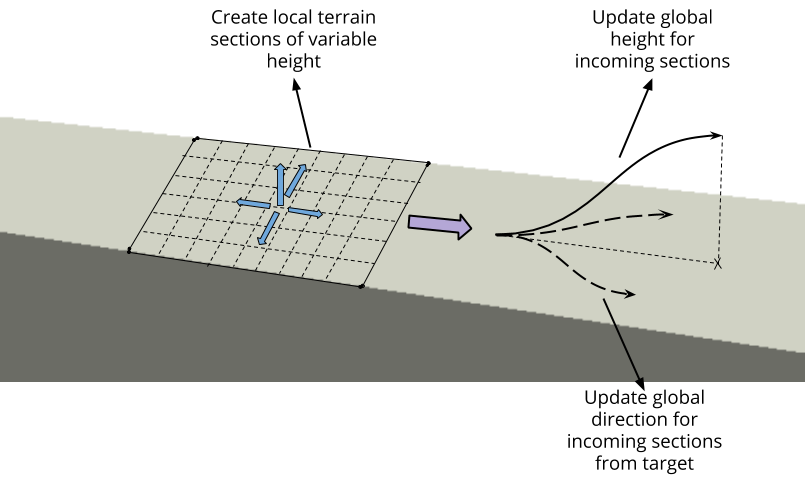
\includegraphics[width=0.85\textwidth]{./chapters/chapter_4/imgs/img_ch4_terrain_parameterization_3.png}
        \caption{A thrid variation of the environments, modifying the terrain in three directions
                 by following a target in 3D}
        \label{fig:ch4_terrain_parameterization_three}
    \end{figure}
}

\newcommand{\figTerrainParameterizationFour}{
    \begin{figure}[!ht]
        \centering
        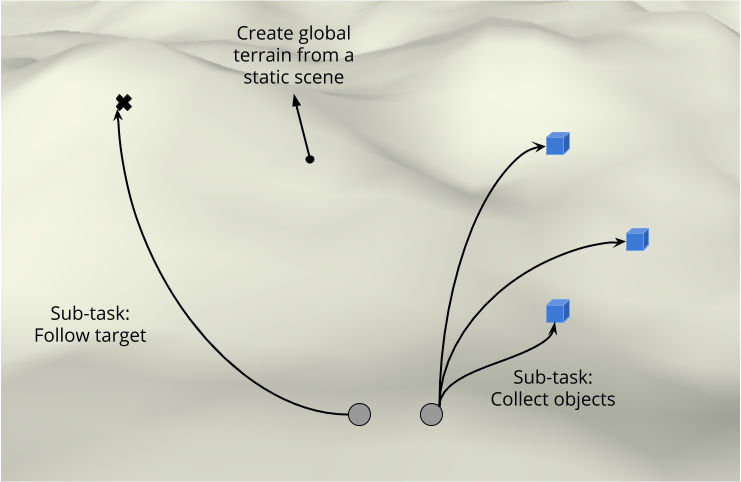
\includegraphics[width=0.85\textwidth]{./chapters/chapter_4/imgs/img_ch4_terrain_parameterization_4.png}
        \caption{A fourth variation of the environments, using static scenes for the terrain
                 and defining sub-tasks for the agent to solve}
        \label{fig:ch4_terrain_parameterization_four}
    \end{figure}
}

\newcommand{\figAgentsExperimentsOne}{
    \begin{figure}[!ht]
        \centering
        \begin{subfigure}[b]{0.48\textwidth}
            \centering
            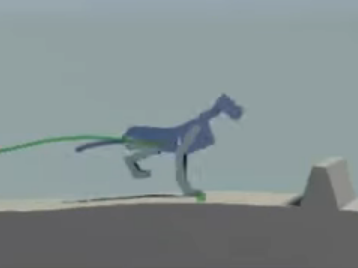
\includegraphics[width=1.0\textwidth]{./chapters/chapter_4/imgs/img_ch4_agent_models_1.png}
            \caption{}
        \end{subfigure}
        \begin{subfigure}[b]{0.48\textwidth}
            \centering
            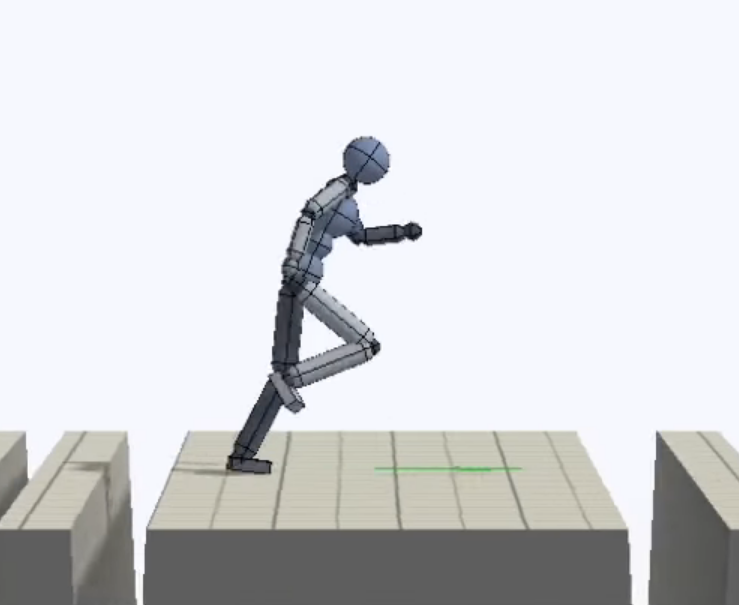
\includegraphics[width=1.0\textwidth]{./chapters/chapter_4/imgs/img_ch4_agent_models_2.png}
            \caption{}
        \end{subfigure}
        \caption{Dog and humanoid models from \citeauthor{TerrainRLSim}}
        \label{fig:ch4_agents_experiments_1}
    \end{figure}
}

\newcommand{\figAgentsExperimentsTwo}{
    \begin{figure}[!ht]
        \centering
        \begin{subfigure}[b]{0.45\textwidth}
            \centering
            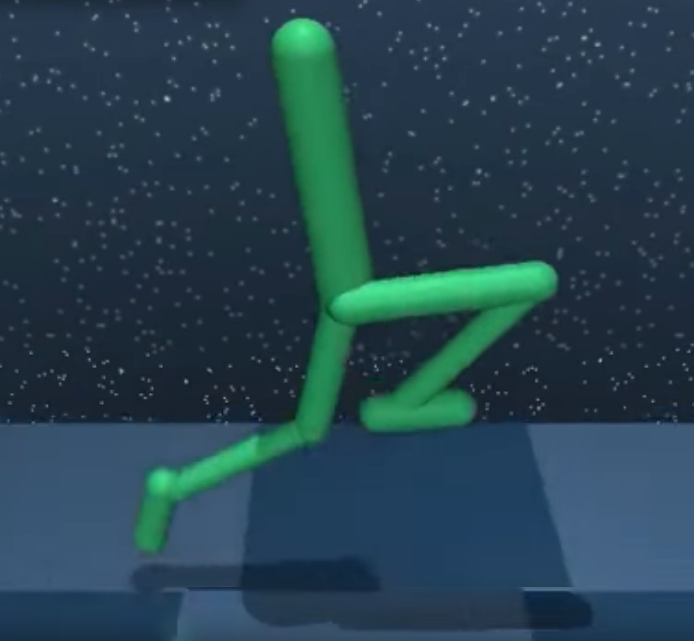
\includegraphics[width=0.9\textwidth]{./chapters/chapter_4/imgs/img_ch4_agent_models_3.png}
            \caption{}
        \end{subfigure}
        \begin{subfigure}[b]{0.45\textwidth}
            \centering
            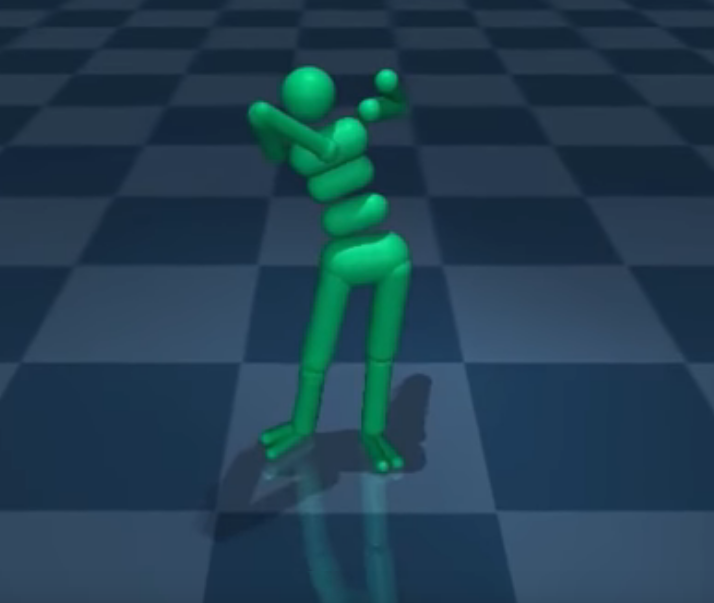
\includegraphics[width=0.9\textwidth]{./chapters/chapter_4/imgs/img_ch4_agent_models_4.png}
            \caption{}
        \end{subfigure}
        \caption{Walker and humanoid models from \citeauthor{Controlsuite}}
        \label{fig:ch4_agents_experiments_2}
    \end{figure}
}

\newcommand{\figAgentsExperimentsThree}{
    \begin{figure}[!ht]
        \centering
        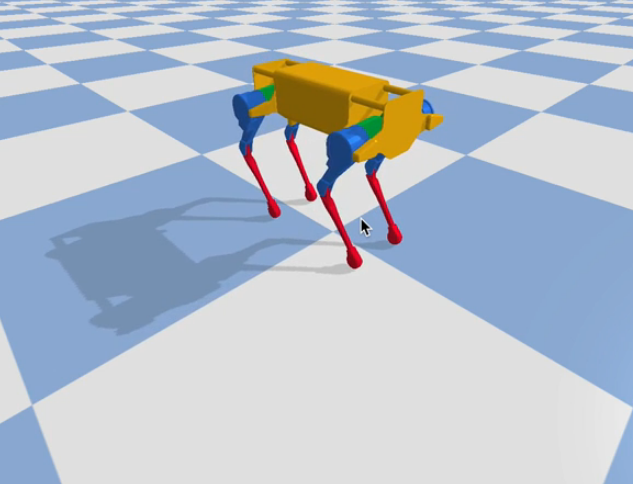
\includegraphics[width=0.8\textwidth]{./chapters/chapter_4/imgs/img_ch4_agent_models_5.png}
        \caption{Agent model for the laikago robot from 
                 \href{http://www.unitree.cc/e/action/ShowInfo.php?classid=6&id=1}{Unitree}, adapted
                 from \citeauthor{PyBullet}}
        \label{fig:ch4_agents_experiments_3}
    \end{figure}
}

\newcommand{\figFrameworkFlow}{
    \begin{figure}[!ht]
        \centering
        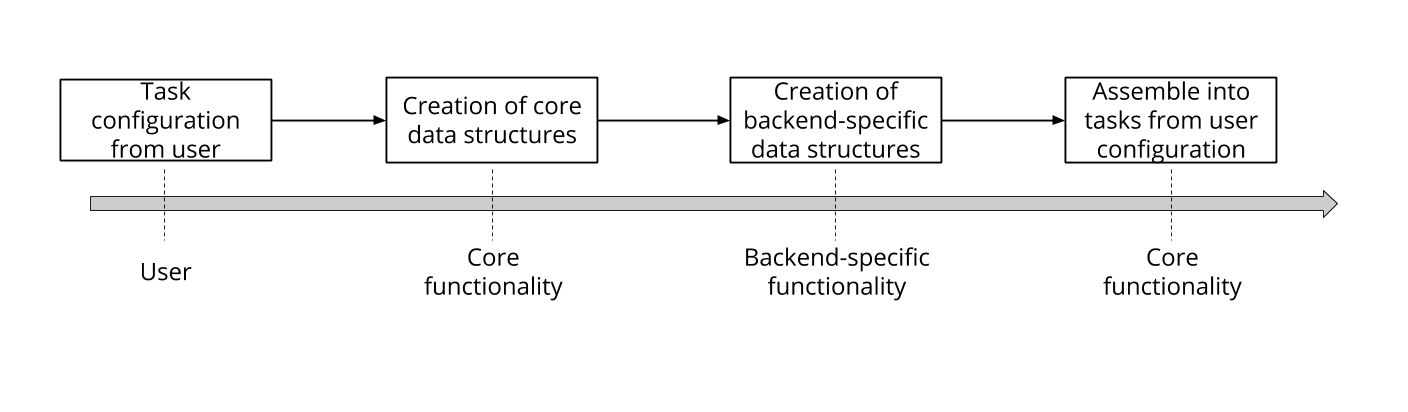
\includegraphics[width=0.9\textwidth]{./chapters/chapter_4/imgs/img_ch4_framework_flow.png}
        \caption{Flow of data in the proposed framework}
        \label{fig:ch4_proposed_framework_flow}
    \end{figure}
}

\newcommand{\figFrameworkArchitecture}{
    \begin{figure}
        \centering
        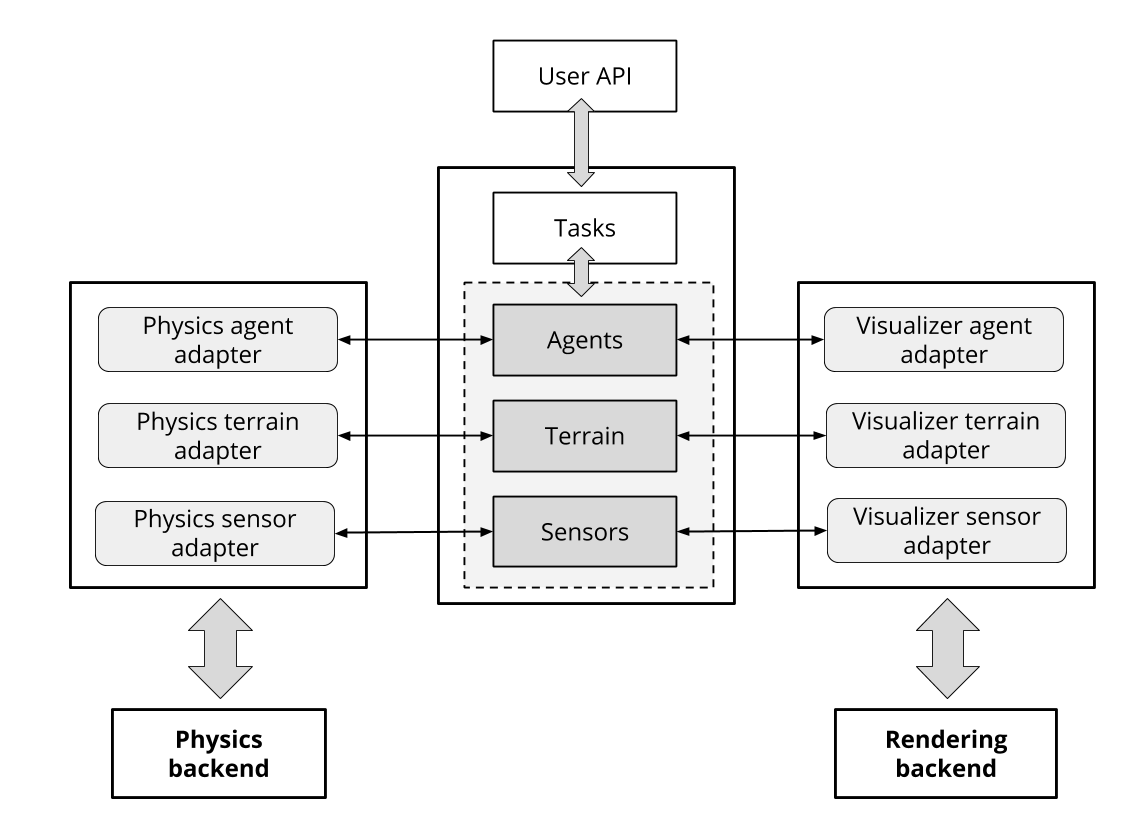
\includegraphics[width=0.9\textwidth]{./chapters/chapter_4/imgs/img_ch4_framework_architecture.png}
        \caption{Architecture of the proposed framework}
        \label{fig:ch4_proposed_framework_architecture}
    \end{figure}
}

\newcommand{\figFrameworkCoreAgent}{
    \begin{figure}[!ht]
        \centering
        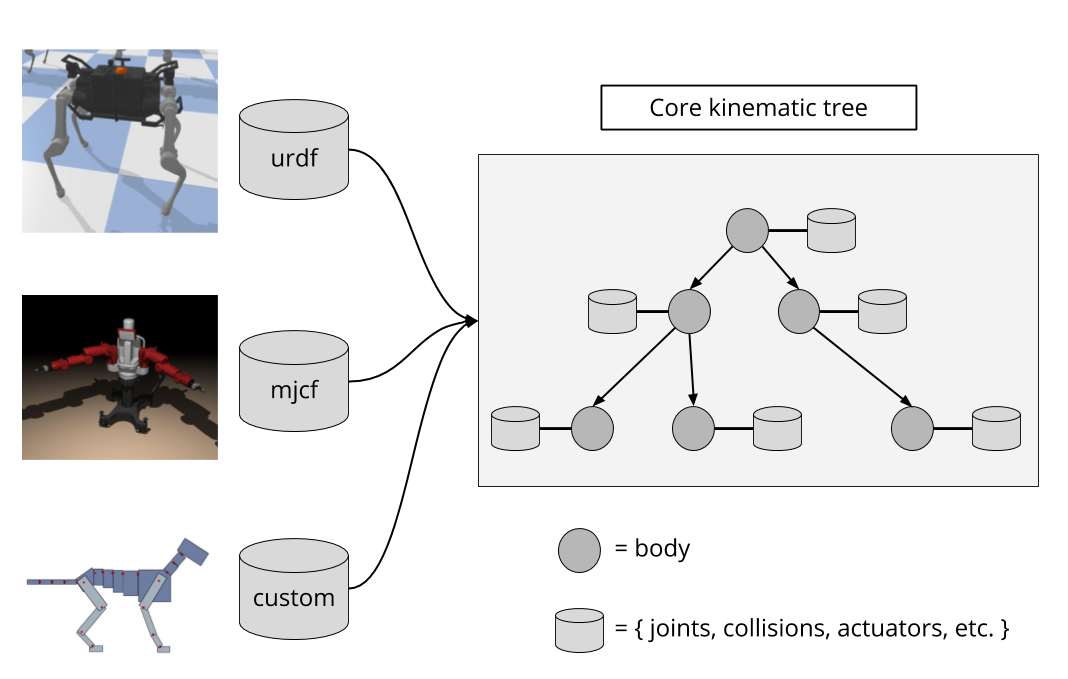
\includegraphics[width=0.9\textwidth]{./chapters/chapter_4/imgs/img_ch4_agents_core.png}
        \caption{Core agent functionality. Model formats are loaded into 
                 the core kinematic tree}
        \label{fig:ch4_core_agent_functionality}
    \end{figure}
}

\newcommand{\figFrameworkCoreTerrain}{
    \begin{figure}[!ht]
        \centering
        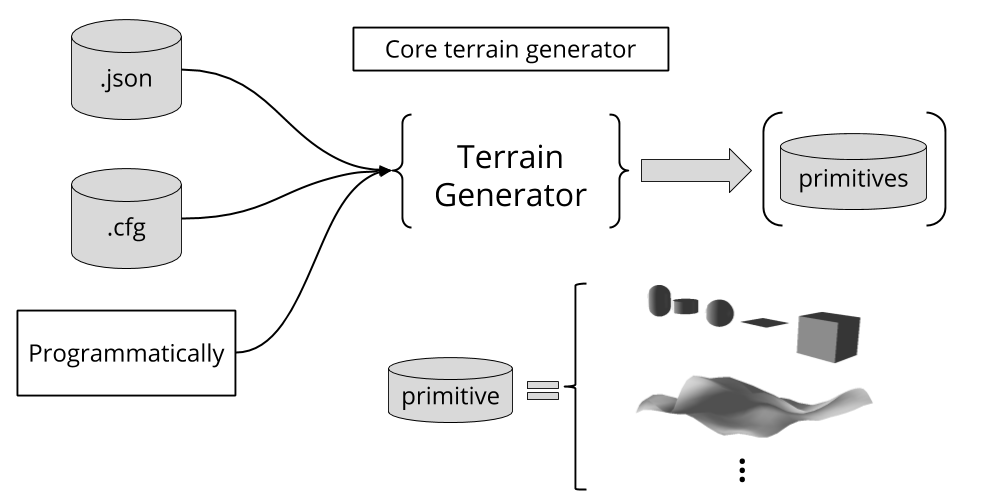
\includegraphics[width=0.9\textwidth]{./chapters/chapter_4/imgs/img_ch4_terrain_core.png}
        \caption{Core terrain functionality. User configuration is passed to the terrain generator
                 and the generator then creates blueprints to be used by the backend.}
        \label{fig:ch4_core_terrain_functionality}
    \end{figure}
}

\newcommand{\figFrameworkCoreSensor}{
    \begin{figure}[!ht]
        \centering
        \begin{subfigure}[b]{0.3\textwidth}
            \centering
            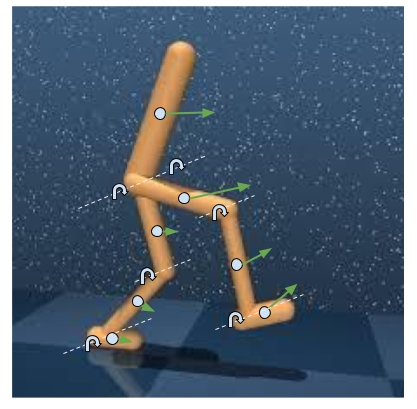
\includegraphics[width=0.9\textwidth]{./chapters/chapter_4/imgs/img_ch4_sensors_core_1.png}
            \caption{}
            \label{fig:ch4_core_sensor_1}
        \end{subfigure}
        \begin{subfigure}[b]{0.3\textwidth}
            \centering
            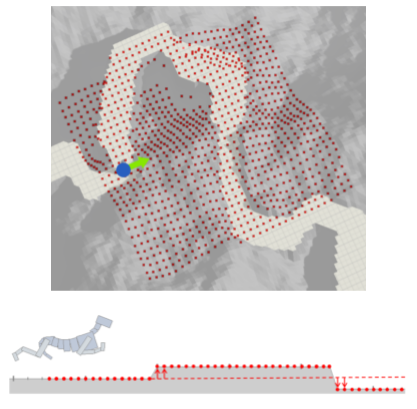
\includegraphics[width=0.9\textwidth]{./chapters/chapter_4/imgs/img_ch4_sensors_core_2.png}
            \caption{}
            \label{fig:ch4_core_sensor_2}
        \end{subfigure}
        \begin{subfigure}[b]{0.3\textwidth}
            \centering
            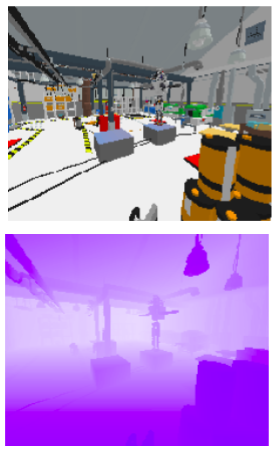
\includegraphics[width=0.9\textwidth]{./chapters/chapter_4/imgs/img_ch4_sensors_core_3.png}
            \caption{}
            \label{fig:ch4_core_sensor_3}
        \end{subfigure}
        \caption{Core sensors functionality. a) Intrinsic readings from joints and bodies (adapted from \cite{DeepmindEmergenceLocomotion}).
                                             b) Extrinsic readings from heightmaps of the terrain (adapted from \citeauthor{DeepLoco} and \citeauthor{DeepTerrainRL}).
                                             c) Extrinsic readings from rgb and depth images of the agent view (adapted from \cite{PyBullet}).}
        \label{fig:ch4_core_sensor_functionality}
    \end{figure}
}

\newcommand{\figBridgePattern}{
    \begin{figure}[!ht]
        \centering
        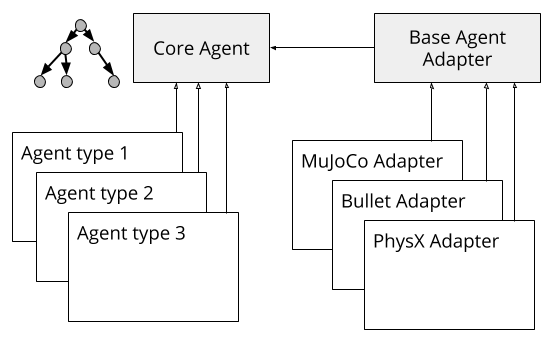
\includegraphics[width=0.9\textwidth]{./chapters/chapter_4/imgs/img_ch4_bridge_pattern.png}
        \caption{Bridge pattern used to decouple agent functionality}
        \label{fig:ch4_bridge_pattern}
    \end{figure}
}

\newcommand{\figRuntimeLibraryLoading}{
    \begin{figure}[!ht]
        \centering
        
\includegraphics[width=0.9\textwidth]{./chapters/chapter_4/imgs/img_ch4_runtime_library_loading.png}
        \caption{Loading specific backend at runtime}
        \label{fig:ch4_runtime_library_loading}
    \end{figure}
}